\documentclass[a4paper, 10pt, twoside]{article}

% Set up page margins using geometry package for two-sided printing.
% The bindingoffset adds extra space on the inner margin (left side on odd pages,
% right side on even pages).
\usepackage[
  a4paper,
  twoside,
  bindingoffset=15mm,       % Space for binding on inner edges
  inner=25mm,               % Inner margin
  outer=20mm,               % Outer margin
  top=20mm,
  bottom=20mm
]{geometry}

% For better typography
\usepackage[T1]{fontenc}
\usepackage[utf8]{inputenc}
\usepackage[ngerman]{babel}
\usepackage{lmodern}

\usepackage{setspace}
\usepackage{amsmath}
\usepackage{amssymb}
\usepackage{enumitem}
\usepackage{minted}
\usepackage{xcolor}
\usepackage{graphicx}
\graphicspath{{Images/}}


% Color Palette 
\definecolor{Clouds}{HTML}{ecf0f1} 

% Minted Settings for Code Blocks
\usemintedstyle{tango} 

\setminted{
  linenos,
  breaklines,
  fontsize=\small,
  bgcolor=Clouds,
  autogobble
}

% Set Space between Lines 
\doublespacing

% ===== DOCUMENT =====
\begin{document}

% ===== FRONT PAGE =====
\begin{titlepage}
    \centering
    {\Huge\bfseries Embedded Systems\par}
    \vspace{1cm}
    {\Large Zusammenfassung\par}
    \vspace{2cm}
    {\large WiSe24/25\par}
    \vfill
    % You can add a logo or graphic here if desired
\end{titlepage}

% ===== TABLE OF CONTENTS =====
\tableofcontents
\clearpage

% ===== MAIN CONTENT =====

\raggedright

\section{I/O Ports}

Ports werden durch 8 Bit Register konfiguriert.

Der ATmega328p hat insgesamt 3 Portbänke (B, C und D).

Ports können auch mehrfach belegt sein!


\subsection{Data Direction Register}

Die Data Direction Register der jeweiligen Ports legen die Richtung fest.

0 = Input (Default), 1 = Output

\vspace{2em}
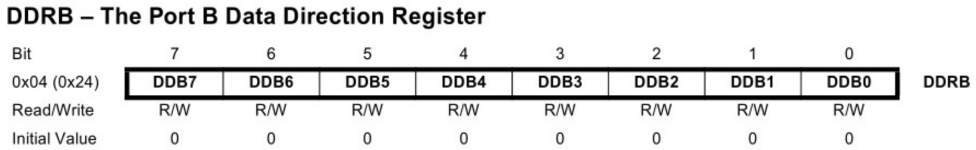
\includegraphics[scale=0.5]{DDRB.png}
\vspace{2em}



\end{document}
